\documentclass[10pt]{article}

\usepackage[margin=1.8cm,top=1.6cm,bottom=1.8cm]{geometry}
\usepackage[table]{xcolor}
\usepackage{tcolorbox}
\tcbuselibrary{breakable}
\usepackage{tikz}
\usetikzlibrary{positioning,arrows.meta}
\usepackage{booktabs}
\usepackage{array}
\usepackage{tabularx}
\usepackage{enumitem}
\usepackage{fontawesome5}
\usepackage{fancyhdr}
\usepackage{hyperref}

\definecolor{adrnavy}{RGB}{19,33,61}
\definecolor{adrteal}{RGB}{0,119,138}
\definecolor{adrslate}{RGB}{92,102,120}
\definecolor{adrbg}{RGB}{247,248,250}
\definecolor{adrgreen}{RGB}{27,120,66}
\definecolor{adrgreenbg}{RGB}{224,241,230}
\definecolor{adramber}{RGB}{158,103,13}
\definecolor{adramberbg}{RGB}{250,235,208}
\definecolor{adrred}{RGB}{163,36,36}
\definecolor{adrredbg}{RGB}{249,225,225}
\definecolor{adrgrey}{RGB}{107,114,128}
\definecolor{adrgreybg}{RGB}{233,235,238}

\hypersetup{
  colorlinks=true,
  linkcolor=adrteal,
  urlcolor=adrteal,
  citecolor=adrteal,
  pdftitle={Nimbus Order Platform -- Architecture Decision Records},
  pdfauthor={Nimbus Platform Engineering}
}

\newtcbox{\badgeAccepted}{on line,arc=2pt,colframe=adrgreen,colback=adrgreenbg,boxrule=0.6pt,left=5pt,right=5pt,top=1.5pt,bottom=1.5pt,fontupper=\bfseries\small\color{adrgreen}}
\newtcbox{\badgeProposed}{on line,arc=2pt,colframe=adramber,colback=adramberbg,boxrule=0.6pt,left=5pt,right=5pt,top=1.5pt,bottom=1.5pt,fontupper=\bfseries\small\color{adramber}}
\newtcbox{\badgeSuperseded}{on line,arc=2pt,colframe=adrred,colback=adrredbg,boxrule=0.6pt,left=5pt,right=5pt,top=1.5pt,bottom=1.5pt,fontupper=\bfseries\small\color{adrred}}
\newtcbox{\badgeDeprecated}{on line,arc=2pt,colframe=adrgrey,colback=adrgreybg,boxrule=0.6pt,left=5pt,right=5pt,top=1.5pt,bottom=1.5pt,fontupper=\bfseries\small\color{adrgrey}}

\newtcolorbox{ctxbox}{breakable,colback=white,colframe=adrteal,coltitle=white,colbacktitle=adrteal,fonttitle=\bfseries,title={\faFile\ Context},fontupper=\small,arc=1pt,boxrule=0.7pt,left=7pt,right=7pt,top=2pt,bottom=2pt,before skip=2pt,after skip=2pt}
\newtcolorbox{decbox}{breakable,colback=white,colframe=adrnavy,coltitle=white,colbacktitle=adrnavy,fonttitle=\bfseries,title={\faCheckCircle\ Decision},fontupper=\small,arc=1pt,boxrule=0.7pt,left=7pt,right=7pt,top=2pt,bottom=2pt,before skip=2pt,after skip=2pt}
\newtcolorbox{consbox}{breakable,colback=white,colframe=adrslate,coltitle=white,colbacktitle=adrslate,fonttitle=\bfseries,title={\faExclamationTriangle\ Consequences},fontupper=\small,arc=1pt,boxrule=0.7pt,left=7pt,right=7pt,top=2pt,bottom=2pt,before skip=2pt,after skip=2pt}
\newtcolorbox{metabox}{breakable,colback=adrbg,colframe=adrteal!45,arc=1pt,boxrule=0.6pt,left=7pt,right=7pt,top=3pt,bottom=3pt,before skip=3pt,after skip=2pt}

\newcommand{\adrheading}[2]{%
  \par\vspace{5pt}%
  {\color{adrnavy}\Large\bfseries #1 \quad\textemdash\quad #2}\par
  \vspace{1pt}
  \noindent\textcolor{adrteal}{\rule{\linewidth}{1.4pt}}\par
  \vspace{1pt}
}

\pagestyle{fancy}
\fancyhf{}
\renewcommand{\headrulewidth}{0.6pt}
\renewcommand{\headrule}{\hbox to\headwidth{\color{adrteal!60}\leaders\hrule height \headrulewidth\hfill}}
\fancyhead[L]{\small\color{adrslate}Nimbus Order Platform --- Decision Register}
\fancyhead[R]{\small\color{adrslate}\thepage}
\fancyfoot[C]{\small\color{adrslate}Internal Engineering Document \textbullet\ Confidential}

\setlist[itemize]{leftmargin=1.3em,itemsep=0pt,topsep=1pt}

\setlength{\parindent}{0pt}
\setlength{\parskip}{2pt}
\renewcommand{\arraystretch}{0.88}

\begin{document}

% ---------- Title banner ----------
\begin{tcolorbox}[colback=adrnavy,colframe=adrnavy,arc=2pt,boxrule=0pt,left=18pt,right=18pt,top=14pt,bottom=14pt]
{\color{white}\Huge\bfseries Architecture Decision Records}\\[4pt]
{\color{adrbg!90}\Large Nimbus Order Platform}\\[8pt]
{\color{white!85!adrbg}\small \faDatabase\ Platform Engineering \quad\textbullet\quad \faUsers\ Maintained by the Architecture Guild \quad\textbullet\quad \faCalendar\ Last reviewed 2025-06-02}
\end{tcolorbox}

\vspace{6pt}
Architecture Decision Records (ADRs) capture the significant, hard-to-reverse technical choices made while building the Nimbus order and fulfillment platform. Each record is immutable once accepted: if circumstances change, we write a new ADR that supersedes the old one rather than editing history. This register is the canonical index --- consult it before proposing an approach that a past decision already ruled on.

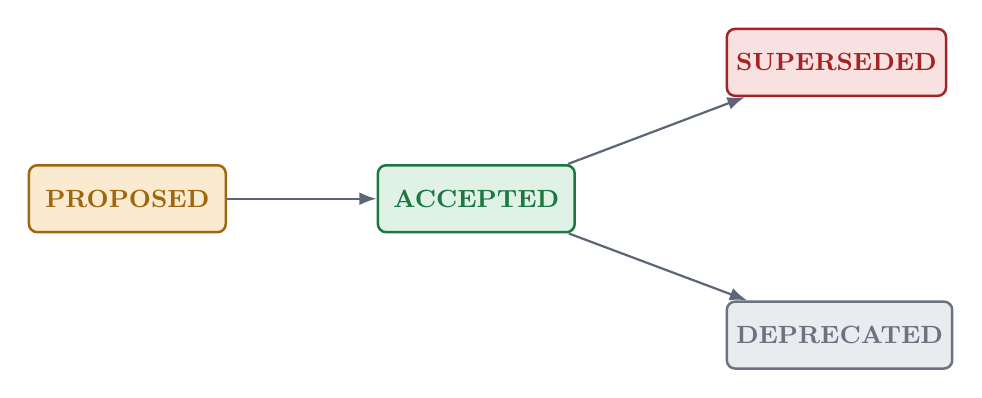
\begin{tikzpicture}[
  node distance=1.1cm and 1.9cm,
  every node/.style={font=\small\bfseries},
  box/.style={rectangle,rounded corners=3pt,draw,minimum width=2.5cm,minimum height=0.85cm,align=center,line width=0.9pt},
  arr/.style={-{Latex[length=2.2mm]},line width=0.8pt,draw=adrslate}
]
\node[box,draw=adramber,fill=adramberbg,text=adramber] (proposed) {PROPOSED};
\node[box,draw=adrgreen,fill=adrgreenbg,text=adrgreen,right=of proposed] (accepted) {ACCEPTED};
\node[box,draw=adrred,fill=adrredbg,text=adrred,above right=0.85cm and 1.9cm of accepted] (superseded) {SUPERSEDED};
\node[box,draw=adrgrey,fill=adrgreybg,text=adrgrey,below right=0.85cm and 1.9cm of accepted] (deprecated) {DEPRECATED};

\draw[arr] (proposed) -- (accepted);
\draw[arr] (accepted) -- (superseded);
\draw[arr] (accepted) -- (deprecated);
\end{tikzpicture}

\vspace{1pt}
{\bfseries\color{adrnavy}Decision Register}\par
\vspace{2pt}
\rowcolors{2}{adrbg}{white}
\begin{tabularx}{\linewidth}{@{}l X l l@{}}
\rowcolor{adrnavy}
{\color{white}\bfseries ID} & {\color{white}\bfseries Title} & {\color{white}\bfseries Status} & {\color{white}\bfseries Date} \\
ADR-0001 & Record architecture decisions as lightweight ADRs & \badgeAccepted{ACCEPTED} & 2024-11-04 \\
ADR-0002 & PostgreSQL as system of record for the order ledger & \badgeAccepted{ACCEPTED} & 2024-11-18 \\
ADR-0003 & Kafka for asynchronous order-fulfillment events & \badgeAccepted{ACCEPTED} & 2025-01-09 \\
ADR-0004 & Adopt gRPC for internal service-to-service calls & \badgeProposed{PROPOSED} & 2025-05-27 \\
ADR-0005 & Retire the legacy SOAP integration layer & \badgeSuperseded{SUPERSEDED} & 2024-09-12 \\
\end{tabularx}


% ================= ADR-0001 =================
\adrheading{ADR-0001}{Record Architecture Decisions as Lightweight ADRs}

\begin{metabox}
\begin{tabularx}{\linewidth}{@{}l X l X@{}}
\textbf{\faCheckCircle\ Status} & \badgeAccepted{ACCEPTED} & \textbf{\faCalendar\ Date} & 2024-11-04 \\
\textbf{\faUsers\ Deciders} & M. Alvarez, R. Okonkwo, S. Bergstrom & \textbf{\faTag\ Tags} & process, governance \\
\textbf{\faLink\ Supersedes} & --- & \textbf{\faLink\ Superseded by} & --- \\
\end{tabularx}
\end{metabox}

\begin{ctxbox}
The order-fulfillment rewrite has grown to nine services and four data stores maintained by three squads. Decisions about data ownership, messaging, and protocol choices were previously discussed in chat threads and design docs that were hard to find six months later. New engineers repeatedly re-opened debates ("why Postgres and not DynamoDB?") that had already been settled, and two squads independently built incompatible retry strategies because neither knew the other's reasoning. We need a durable, low-overhead record of significant technical decisions and the context behind them.
\end{ctxbox}

\begin{decbox}
We will record every architecturally significant decision as a short Markdown file under \texttt{/docs/adr/}, numbered sequentially (\texttt{NNNN-title.md}), following this five-part shape: \textit{Status}, \textit{Context}, \textit{Decision}, \textit{Consequences}, \textit{Alternatives Considered}. Records are immutable once merged to \texttt{main}. A decision is superseded, never edited: a new ADR is written and the old one's status changes to \textbf{Superseded by ADR-NNNN}. Any change to a service boundary, data-ownership model, communication protocol, or a dependency that is expensive to reverse requires an ADR before implementation begins.
\end{decbox}

\begin{consbox}
\noindent
\begin{minipage}[t]{0.48\linewidth}
\textbf{\textcolor{adrgreen}{Positive}}
\begin{itemize}
\item[\textcolor{adrgreen}{\faCheckCircle}] New hires read the register instead of re-litigating settled debates.
\item[\textcolor{adrgreen}{\faCheckCircle}] Reviewing an ADR PR is a five-minute task, so the process survives contact with deadlines.
\item[\textcolor{adrgreen}{\faCheckCircle}] Postmortems can cite the exact reasoning that led to an incident-adjacent choice.
\end{itemize}
\end{minipage}\hfill
\begin{minipage}[t]{0.48\linewidth}
\textbf{\textcolor{adrred}{Negative}}
\begin{itemize}
\item[\textcolor{adrred}{\faTimesCircle}] Adds a review step before implementation on decisions that are genuinely urgent.
\item[\textcolor{adrred}{\faTimesCircle}] Requires discipline to keep the register current as squads reorganize.
\end{itemize}
\end{minipage}
\end{consbox}

\textbf{\color{adrnavy}Alternatives Considered}\par
\vspace{1pt}
\rowcolors{2}{adrbg}{white}
\small
\begin{tabularx}{\linewidth}{@{}p{2.6cm} X X l@{}}
\rowcolor{adrslate}
{\color{white}\bfseries Option} & {\color{white}\bfseries Pros} & {\color{white}\bfseries Cons} & {\color{white}\bfseries Verdict} \\
Confluence wiki pages & Familiar tooling, rich formatting & Drifts from code, no PR review, hard to search & Rejected \\
No formal record & Zero process overhead & Already causing repeated debates and drift & Rejected \\
Full RFC process & Deep stakeholder sign-off & Too heavyweight for day-to-day decisions & Rejected \\
Markdown ADRs in-repo & Versioned with code, reviewed via PR & Requires discipline to keep terse & \textbf{Chosen} \\
\end{tabularx}
\normalsize


% ================= ADR-0002 =================
\adrheading{ADR-0002}{PostgreSQL as System of Record for the Order Ledger}

\begin{metabox}
\begin{tabularx}{\linewidth}{@{}l X l X@{}}
\textbf{\faCheckCircle\ Status} & \badgeAccepted{ACCEPTED} & \textbf{\faCalendar\ Date} & 2024-11-18 \\
\textbf{\faUsers\ Deciders} & R. Okonkwo, S. Bergstrom, T. Lindqvist & \textbf{\faTag\ Tags} & data, ledger, postgres \\
\textbf{\faLink\ Supersedes} & --- & \textbf{\faLink\ Superseded by} & --- \\
\end{tabularx}
\end{metabox}

\begin{ctxbox}
The order ledger records every state transition of an order --- placed, paid, packed, shipped, refunded --- and is the source of truth for finance reconciliation and dispute handling. It requires strict transactional guarantees: two writers must never both mark the same order ``paid,'' and a partial write (payment captured, ledger not updated) is unacceptable. Write volume is moderate (peak \textasciitilde900 writes/sec during flash sales) but correctness matters more than raw throughput. The team evaluated DynamoDB, already used at Nimbus for the session store, against PostgreSQL, already run in production for the catalog service.
\end{ctxbox}

\begin{decbox}
We will use PostgreSQL 15 (Vertex RDS, Multi-AZ) as the system of record for the order ledger. Each order-state transition is written inside a single ACID transaction alongside its audit-log row, using \texttt{SELECT ... FOR UPDATE} to serialize concurrent transitions on the same order. Read replicas absorb the reporting and support-tooling read paths so writes are never contended by analytics queries.
\end{decbox}

\begin{consbox}
\noindent
\begin{minipage}[t]{0.48\linewidth}
\textbf{\textcolor{adrgreen}{Positive}}
\begin{itemize}
\item[\textcolor{adrgreen}{\faCheckCircle}] Multi-row ACID transactions make the ``paid + ledger'' invariant trivial to enforce.
\item[\textcolor{adrgreen}{\faCheckCircle}] Existing on-call runbooks and backup tooling already cover Postgres.
\item[\textcolor{adrgreen}{\faCheckCircle}] Read replicas isolate analytics load from the write path at negligible cost.
\end{itemize}
\end{minipage}\hfill
\begin{minipage}[t]{0.48\linewidth}
\textbf{\textcolor{adrred}{Negative}}
\begin{itemize}
\item[\textcolor{adrred}{\faTimesCircle}] Vertical scaling ceiling is lower than DynamoDB; revisit if writes exceed \textasciitilde5k/sec.
\item[\textcolor{adrred}{\faTimesCircle}] Multi-AZ failover adds \textasciitilde30s of write unavailability during an RDS event.
\end{itemize}
\end{minipage}
\end{consbox}

\textbf{\color{adrnavy}Alternatives Considered}\par
\vspace{1pt}
\rowcolors{2}{adrbg}{white}
\small
\begin{tabularx}{\linewidth}{@{}p{2.6cm} X X l@{}}
\rowcolor{adrslate}
{\color{white}\bfseries Option} & {\color{white}\bfseries Pros} & {\color{white}\bfseries Cons} & {\color{white}\bfseries Verdict} \\
DynamoDB & Near-infinite write scaling, low ops overhead & Multi-item transactions are limited (25 items, single region); weaker fit for ledger invariants & Rejected \\
Aurora PostgreSQL & Faster failover (\textasciitilde10s), storage auto-scaling & Higher cost, another platform to certify at short notice & Deferred \\
Event-sourced store (custom) & Full history is a first-class model & Significant build cost; duplicates what a WAL-backed RDBMS gives for free & Rejected \\
RDS PostgreSQL 15 & Strong consistency, team already runs it in prod & Scaling ceiling lower than DynamoDB & \textbf{Chosen} \\
\end{tabularx}
\normalsize


% ================= ADR-0003 =================
\adrheading{ADR-0003}{Kafka for Asynchronous Order-Fulfillment Events}

\begin{metabox}
\begin{tabularx}{\linewidth}{@{}l X l X@{}}
\textbf{\faCheckCircle\ Status} & \badgeAccepted{ACCEPTED} & \textbf{\faCalendar\ Date} & 2025-01-09 \\
\textbf{\faUsers\ Deciders} & M. Alvarez, T. Lindqvist, P. Nakamura & \textbf{\faTag\ Tags} & messaging, kafka, fulfillment \\
\textbf{\faLink\ Supersedes} & --- & \textbf{\faLink\ Superseded by} & --- \\
\end{tabularx}
\end{metabox}

\begin{ctxbox}
Once an order is marked ``paid'' in the ledger (ADR-0002), five downstream services must react: inventory reservation, warehouse routing, invoicing, fraud re-scoring, and customer notification. Today the order service calls each synchronously over HTTP, so placement blocks on the slowest of the five, and a single unavailable service (fraud re-scoring, most often) degrades checkout latency for every order, not just the ones it flags. We need to decouple ``paid'' from ``every downstream system has processed it,'' while keeping strict per-order ordering.
\end{ctxbox}

\begin{decbox}
We will publish order lifecycle events (\texttt{order.paid}, \texttt{order.cancelled}, \texttt{order.refunded}, \texttt{order.shipped}) to an Apache Kafka topic (\texttt{MSK}, 12 partitions, keyed by \texttt{order\_id}) immediately after the ledger transaction commits, using the transactional outbox pattern to guarantee the event publishes if and only if the ledger write succeeded. Downstream services consume independently with their own consumer groups and offsets, so a slow or down consumer no longer blocks checkout or any other consumer.
\end{decbox}

\begin{consbox}
\noindent
\begin{minipage}[t]{0.48\linewidth}
\textbf{\textcolor{adrgreen}{Positive}}
\begin{itemize}
\item[\textcolor{adrgreen}{\faCheckCircle}] Checkout latency no longer depends on the slowest downstream consumer.
\item[\textcolor{adrgreen}{\faCheckCircle}] A down consumer catches up from its committed offset with zero data loss.
\item[\textcolor{adrgreen}{\faCheckCircle}] New consumers (a future loyalty-points service) can subscribe without touching the order service.
\end{itemize}
\end{minipage}\hfill
\begin{minipage}[t]{0.48\linewidth}
\textbf{\textcolor{adrred}{Negative}}
\begin{itemize}
\item[\textcolor{adrred}{\faTimesCircle}] Introduces eventual consistency; support tooling must show ``processing'' states honestly.
\item[\textcolor{adrred}{\faTimesCircle}] Outbox pattern adds a polling publisher process to operate and monitor.
\item[\textcolor{adrred}{\faTimesCircle}] Squads must learn consumer-group rebalancing and offset-management failure modes.
\end{itemize}
\end{minipage}
\end{consbox}

\textbf{\color{adrnavy}Alternatives Considered}\par
\vspace{1pt}
\rowcolors{2}{adrbg}{white}
\small
\begin{tabularx}{\linewidth}{@{}p{2.6cm} X X l@{}}
\rowcolor{adrslate}
{\color{white}\bfseries Option} & {\color{white}\bfseries Pros} & {\color{white}\bfseries Cons} & {\color{white}\bfseries Verdict} \\
Synchronous HTTP (status quo) & Simple mental model, immediate feedback & Couples checkout latency to five downstream services & Rejected \\
SQS standard queues & Fully managed, minimal ops & No per-order ordering guarantee across consumers & Rejected \\
SQS FIFO queues & Ordering per message group & Throughput ceiling too low for flash-sale peaks & Rejected \\
Apache Kafka (MSK) & Ordered per partition, high throughput, replayable & Team must operate consumer-group tooling & \textbf{Chosen} \\
\end{tabularx}
\normalsize


% ================= ADR-0004 =================
\adrheading{ADR-0004}{Adopt gRPC for Internal Service-to-Service Calls}

\begin{metabox}
\begin{tabularx}{\linewidth}{@{}l X l X@{}}
\textbf{\faCheckCircle\ Status} & \badgeProposed{PROPOSED} & \textbf{\faCalendar\ Date} & 2025-05-27 \\
\textbf{\faUsers\ Deciders} & S. Bergstrom, P. Nakamura & \textbf{\faTag\ Tags} & networking, grpc, latency \\
\textbf{\faLink\ Supersedes} & --- & \textbf{\faLink\ Superseded by} & --- \\
\end{tabularx}
\end{metabox}

\begin{ctxbox}
Inventory reservation calls warehouse routing synchronously on the hot path, and profiling from the April load test shows JSON serialization and HTTP/1.1 connection churn account for \textasciitilde22ms of the \textasciitilde140ms call, second only to the database round trip. Nine services now make 40+ internal REST calls per order, and each pair invented its own retry and error-envelope conventions --- flagged twice by on-call as a source of confusion during incidents.
\end{ctxbox}

\begin{decbox}
We propose adopting gRPC over HTTP/2 for internal, synchronous service-to-service calls, starting with the inventory-to-warehouse-routing path. Contracts are defined in Protocol Buffers and published from a shared \texttt{proto/} repository with generated stubs per language. Timeouts, retries, and error codes follow one shared interceptor library instead of being reinvented per service pair. Public-facing APIs are explicitly out of scope and remain REST/JSON.
\end{decbox}

\begin{consbox}
\noindent
\begin{minipage}[t]{0.48\linewidth}
\textbf{\textcolor{adrgreen}{Positive}}
\begin{itemize}
\item[\textcolor{adrgreen}{\faCheckCircle}] Binary protobuf plus HTTP/2 multiplexing removed \textasciitilde18ms from the same call in a spike.
\item[\textcolor{adrgreen}{\faCheckCircle}] Shared \texttt{.proto} contracts catch breaking schema changes at build time, not in production.
\item[\textcolor{adrgreen}{\faCheckCircle}] One retry/timeout/error-code convention replaces nine bespoke ones.
\end{itemize}
\end{minipage}\hfill
\begin{minipage}[t]{0.48\linewidth}
\textbf{\textcolor{adrred}{Negative}}
\begin{itemize}
\item[\textcolor{adrred}{\faTimesCircle}] Debugging with \texttt{curl} disappears; engineers need \texttt{grpcurl} and protobuf tooling.
\item[\textcolor{adrred}{\faTimesCircle}] Load balancers and the service mesh need HTTP/2-aware configuration.
\item[\textcolor{adrred}{\faTimesCircle}] Migration is per-endpoint and will run for several quarters alongside REST.
\end{itemize}
\end{minipage}
\end{consbox}

\textbf{\color{adrnavy}Alternatives Considered}\par
\vspace{1pt}
\rowcolors{2}{adrbg}{white}
\small
\begin{tabularx}{\linewidth}{@{}p{2.6cm} X X l@{}}
\rowcolor{adrslate}
{\color{white}\bfseries Option} & {\color{white}\bfseries Pros} & {\color{white}\bfseries Cons} & {\color{white}\bfseries Verdict} \\
Keep REST/JSON & No migration cost, universally debuggable & Serialization and connection overhead stays on the hot path & Rejected \\
GraphQL federation & Flexible querying for aggregators & Solves a read-shaping problem we do not have & Rejected \\
gRPC over HTTP/2 & Lower latency, typed contracts, shared tooling & Steeper learning curve, mesh reconfiguration & \textbf{Proposed} \\
\end{tabularx}
\normalsize

\vspace{2pt}
\begin{tcolorbox}[colback=adramberbg,colframe=adramber,arc=1pt,boxrule=0.7pt,left=8pt,right=8pt,top=5pt,bottom=5pt]
\small\textbf{\faExclamationTriangle\ Open question:} pilot on the inventory~$\rightarrow$~warehouse-routing path for one release cycle before deciding whether to migrate the remaining eight call sites. Review scheduled for 2025-08-15.
\end{tcolorbox}


% ================= ADR-0005 =================
\adrheading{ADR-0005}{Retire the Legacy SOAP Integration Layer}

\begin{metabox}
\begin{tabularx}{\linewidth}{@{}l X l X@{}}
\textbf{\faCheckCircle\ Status} & \badgeSuperseded{SUPERSEDED} & \textbf{\faCalendar\ Date} & 2024-09-12 \\
\textbf{\faUsers\ Deciders} & R. Okonkwo, M. Alvarez & \textbf{\faTag\ Tags} & integration, legacy, soap \\
\textbf{\faLink\ Supersedes} & --- & \textbf{\faLink\ Superseded by} & ADR-0003 \\
\end{tabularx}
\end{metabox}

\begin{ctxbox}
The original Vertex-era order pipeline integrated with the warehouse-management system via a SOAP/XML interface built in 2019. It requires a stateful adapter process, XML schema validation adds \textasciitilde40ms per call, and the WSDL has not been updated by the warehouse vendor since 2021, so every schema drift on their end has been patched with brittle XSLT transforms on ours. Two production incidents in Q2 2024 traced back to the adapter silently dropping malformed messages instead of raising an alert.
\end{ctxbox}

\begin{decbox}
We decided to decommission the SOAP adapter and replace warehouse notifications with an event published to the (then newly proposed) order-events stream, to be consumed directly by the warehouse-routing service. This decision was folded into and formally superseded by ADR-0003, which generalized the same event-driven approach to all five downstream consumers rather than special-casing warehouse routing alone. The SOAP adapter was fully decommissioned on 2025-02-03 once ADR-0003 shipped to production.
\end{decbox}

\begin{consbox}
\noindent
\begin{minipage}[t]{0.48\linewidth}
\textbf{\textcolor{adrgreen}{Positive}}
\begin{itemize}
\item[\textcolor{adrgreen}{\faCheckCircle}] Removed \textasciitilde40ms of XML validation latency and a full adapter process to operate.
\item[\textcolor{adrgreen}{\faCheckCircle}] Malformed-message failures now raise a consumer-lag alert instead of failing silently.
\end{itemize}
\end{minipage}\hfill
\begin{minipage}[t]{0.48\linewidth}
\textbf{\textcolor{adrred}{Negative}}
\begin{itemize}
\item[\textcolor{adrred}{\faTimesCircle}] Cutover required a two-week dual-write period to validate parity before decommissioning.
\end{itemize}
\end{minipage}
\end{consbox}

\end{document}
